\documentclass[12pt]{article}

%%%%%%%%%%%%%%%%%%%%%%%%%%%%%%%%%%%%%%%%%%%%%%%%%%%%%%%%%%%%%%%%%%%%%%%%%%%%%%%%%%%%%%%%%%%%%%%%%%%%
% Math
\usepackage{fancyhdr} 
\usepackage{amsfonts}
\usepackage{amsmath}
\usepackage{amssymb}
\usepackage{amsthm}
%\usepackage{dsfont}

%%%%%%%%%%%%%%%%%%%%%%%%%%%%%%%%%%%%%%%%%%%%%%%%%%%%%%%%%%%%%%%%%%%%%%%%%%%%%%%%%%%%%%%%%%%%%%%%%%%%
% Macros
\usepackage{calc}

%%%%%%%%%%%%%%%%%%%%%%%%%%%%%%%%%%%%%%%%%%%%%%%%%%%%%%%%%%%%%%%%%%%%%%%%%%%%%%%%%%%%%%%%%%%%%%%%%%%%
% Commands and Custom Variables	
\newcommand{\problem}[1]{\hspace{-4 ex} \large \textbf{Problem #1} }
\let\oldemptyset\emptyset
\let\emptyset\varnothing
\newcommand{\norm}[1]{\left\lVert#1\right\rVert}
\newcommand{\sint}{\text{s}\kern-5pt\int}
\newcommand{\powerset}{\mathcal{P}}
\renewenvironment{proof}{\hspace{-4 ex} \emph{Proof}:}{\qed}
\newcommand{\RR}{\mathbb{R}}
\newcommand{\NN}{\mathbb{N}}
\newcommand{\QQ}{\mathbb{Q}}
\newcommand{\ZZ}{\mathbb{Z}}
\newcommand{\CC}{\mathbb{C}}
\renewcommand{\Re}{\operatorname{Re}}
\renewcommand{\Im}{\operatorname{Im}}


%%%%%%%%%%%%%%%%%%%%%%%%%%%%%%%%%%%%%%%%%%%%%%%%%%%%%%%%%%%%%%%%%%%%%%%%%%%%%%%%%%%%%%%%%%%%%%%%%%%%
%page
\usepackage[margin=1in]{geometry}
\usepackage{setspace}
%\doublespacing
\allowdisplaybreaks
\pagestyle{fancy}
\fancyhf{}
\rhead{Shaw \space \thepage}
\setlength\parindent{0pt}

%%%%%%%%%%%%%%%%%%%%%%%%%%%%%%%%%%%%%%%%%%%%%%%%%%%%%%%%%%%%%%%%%%%%%%%%%%%%%%%%%%%%%%%%%%%%%%%%%%%%
%Code
\usepackage{listings}
\usepackage{courier}
\lstset{
	language=Python,
	showstringspaces=false,
	formfeed=newpage,
	tabsize=4,
	commentstyle=\itshape,
	basicstyle=\ttfamily,
}

%%%%%%%%%%%%%%%%%%%%%%%%%%%%%%%%%%%%%%%%%%%%%%%%%%%%%%%%%%%%%%%%%%%%%%%%%%%%%%%%%%%%%%%%%%%%%%%%%%%%
%Images
\usepackage{graphicx}
\graphicspath{ {images/} }
\usepackage{float}

%tikz
\usepackage[utf8]{inputenc}
\usepackage{pgfplots}
\usepgfplotslibrary{groupplots}

%%%%%%%%%%%%%%%%%%%%%%%%%%%%%%%%%%%%%%%%%%%%%%%%%%%%%%%%%%%%%%%%%%%%%%%%%%%%%%%%%%%%%%%%%%%%%%%%%%%%
%Hyperlinks
%\usepackage{hyperref}
%\hypersetup{
%	colorlinks=true,
%	linkcolor=blue,
%	filecolor=magenta,      
%	urlcolor=cyan,
%}

\begin{document}
	\thispagestyle{empty}
	
	\begin{flushright}
		Sage Shaw \\
		m566 - Spring 2018 \\
		\today
	\end{flushright}
	
{\large \textbf{HW - Chapter 6}}\bigbreak

\problem{4 (a)} Given data $\{(t_i,z_1)\}_{i=0}^m$, the model $u(t) = \gamma_1 e^{\gamma_2 t}$ cannot directly be fit to said data using the techniques given in this chapter, because the parameters are not linear combinations of functions of the data.

\bigbreak
\problem{4 (b)} Convert the model into a linear one and fit it to the data below.

\begin{center}
	\begin{tabular}{|c|c|c|c|}
		\hline
		$i$&1&2&3\\ \hline
		$t_i$&0.0&1.0&2.0\\ \hline
		$z_i$&$e^{0.1}$&$e^{0.9}$&$e^{2}$\\ \hline
	\end{tabular}
\end{center}

The model above can be rewritten as $\ln(u(t)) = \ln(\gamma_1) + \gamma_2 t$. Using this representation we can construct an overdetermined linear system.
$$
%L^{-1} = 
\begin{bmatrix}
1 & t_1\\
1 & t_2\\
1 & t_3
\end{bmatrix}
\begin{bmatrix}
ln(\gamma_1)\\
\gamma_2
\end{bmatrix}
=
\begin{bmatrix}
ln(z_1)\\
ln(z_2)\\
ln(z_3)
\end{bmatrix}
%= L^\prime
$$

Applying a least squared method we find that the parameters of best fit are $\gamma_1 = 1.0512711$ and $\gamma_2 = 0.95$. This exponential regression can be seen in the plot below along with our data. The code that generated these results can be found in the appendix.

\begin{figure}[H]
	\caption{Data points in green and the exponential regression in blue.}
	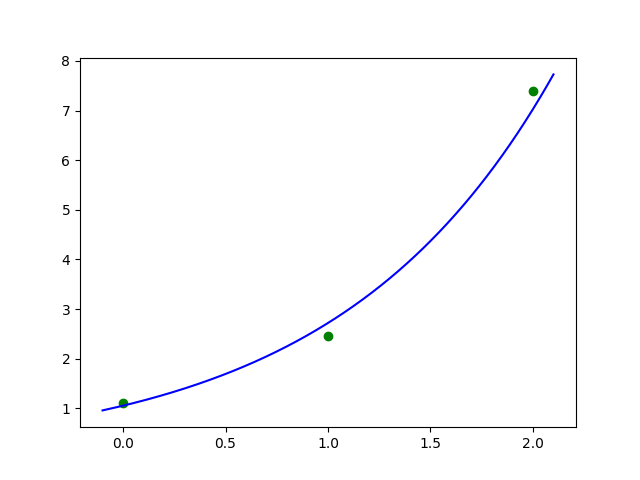
\includegraphics[width=.75\textwidth]{hw1_figure_1.png}
	\label{p1_T_err}
	\centering
\end{figure}

\problem{5 (a)} To illustrate why the LU decomposition cannot be used in the same way as the QR for determining the least squares solution. Assuming we seek a solution to the system $A_{m\times n}x_{n \times 1} = b_{m \times 1}$ and that we have the QR decomposition of $A$ in the form $A = Q_{m \times m} \begin{bmatrix} R_{n \times n} \\ 0\end{bmatrix}$ we can find the least squares by looking for a minimization of the residual (or equivalently the square of the residual)
\begin{align*}
	\norm{r}^2 & = \norm{b-Ax}^2 \\
	& = \norm{b- Q\begin{bmatrix} R_{n \times n} \\ 0\end{bmatrix}x}^2 \\
	& = \norm{Q(Q^Tb - \begin{bmatrix} R_{n \times n} \\ 0\end{bmatrix}x)}^2 \\
	& = \norm{Q^Tb - \begin{bmatrix} R_{n \times n} \\ 0\end{bmatrix}x}^2 \text{\ \ \ \ \ \ (*)}
\end{align*}
Then letting $Q^Tb = \begin{bmatrix} c \\ d\end{bmatrix}$ we continue
\begin{align*}
	& = \norm{\begin{bmatrix} c \\ d\end{bmatrix} - \begin{bmatrix} R_{n \times n} \\ 0\end{bmatrix}x}^2 \\
	& = \norm{c-Rx}^2 + \norm{d}^2
\end{align*}
Minimizing this quantity is equivalent to minimizing $\norm{c-Rx}^2$. The minimum of this is $0$ and the vector $x$ that minimizes it is simply the solution to $Rx = c$. \bigbreak

This method does not work with the LU decomposition instead because it relies on the step (*) above. This steps follows because orthogonal matrices preserve vector norms. This is not necessarily the case for the lower triangular matrix $L$ in general.

%%Suppose one generalized the LU decomposition to full rank matrices of size $m \times n$ for $m>n$. Since $m \ne n$ at least one of the matrices $L \in \RR^{m \times k}$ or $U\in \RR^{k \times n}$ must not be square. If $L$ is not square then the initial forward substitution will fail since the system is over determined. If $U$ is not square a similar situation arises in the back substitution. It should be noted that if $k<n$ then $\text{Rank}(LU) \le k < n$.

\bigbreak
\problem{5 (b)} Using the pseudo-inverse to solve for least squares we are really solving the linear system $(A^TA)x=A^Tb$. This system has a condition number of $\kappa((A^TA)^{-1}) = \kappa(A)^2$. Using the QR method $Rx = Q^Tb$ we have a condition number $\kappa(R) = \kappa(A)$ which is generally better. The step where this improvement is made is marked below
\begin{align*}
	x & = (A^TA)^{-1}A^Tb \\
	& = ((QR)^TQR)^{-1}(QR)^Tb \\
	& = (R^TQ^TQR)^{-1}R^TQ^Tb \\
	& = (R^TR)^{-1}R^TQ^Tb \\
	& = R^{-1}R^{-T}R^TQ^Tb \text{\ \ \ \ \ \ (*)} \\
	& = R^{-1}Q^Tb
\end{align*}

Before step (*) above, we have the implicit system $R^TRx = R^TQ^Tb$ which has a condition number of $\kappa{(R^TR)} = \kappa(A)^2$. After that step we have the implicit system $Rx = Q^Tb$ which as stated before has the condition number $\kappa(A)$.

\bigbreak
\problem{6 (a)} 

\begin{proof} First recall that if $A$ has full rank then $\text{Rank}(AB) = \text{Rank}(B)$. \bigbreak
	Note that $Q$ is orthogonal so $Q^{-1} = Q^T$ exists and $Q$ is full rank. Thus $\text{Rank}(A) = \text{Rank}(R)$. Since $R$ is upper triangular $\text{det}(R) = \prod\limits_{i=1}^n r_{ii}$. Thus $R$ is full rank (i.e. not singular) if and only if its diagonal entries are all non-zero. Thus $A$ has full column rank if and only if the diagonal entries of $R$ are all-non zero.
\end{proof}

\bigbreak
\problem{6 (b)} Since $I \in \RR^{n\times n}$ is non-singular, $\text{Rank}(Q) = n$. Thus $\text{Rank}(A) = \text{Rank}(R)$. The rest follows as in the previous proof.

\bigbreak

\problem{7} We would like to find values $r_{1,1}, r_{1,2}, r_{2,2}, q_{1,1}, q_{1,1}, q_{1,1}$, and $q_{1,1}$ in terms of $a_{i,j}$ such that 
\begin{align*}
	\begin{bmatrix}
	a_{1,1} & a_{1,2} \\
	a_{2,1} & a_{2,2}
	\end{bmatrix}
	=
	\begin{bmatrix}
	q_{1,1} & q_{1,2} \\
	q_{2,1} & q_{2,2}
	\end{bmatrix}
	\begin{bmatrix}
		r_{1,1} & r_{1,2} \\
		0 & r_{2,2}
	\end{bmatrix}
\end{align*}
with the additional constraint that the matrix formed by the $q_{i,j}$ elements is orthonormal. 

\bigbreak

We will first approach this using vectors and then substitute the constituent elements. (Note that we will use $a_i$ to refer to the column vector $\begin{bmatrix}a_{1,i} & a_{2,i} \end{bmatrix}^T$.) In vector form this is
\begin{align*}
	\begin{bmatrix} a_1 & a_2 \end{bmatrix} = \begin{bmatrix} q_1 & q_2 \end{bmatrix} = \begin{bmatrix} r_{1,1} & r_{1,2} \\ & r_{2,2} \end{bmatrix}
\end{align*}
or
\begin{align*}
	a_1 = & r_{1,1}q_1 & a_2 = & r_{1,2}q_1 + r_{2,2}q_2
\end{align*}
Since $\norm{q_1} = 1$ we know that $r_{1,1} = \norm{a_1}$ and then that $q_1 = \frac{1}{\norm{a_1}}a_1$. This gives us the first three of our unknowns
\begin{align}
	r_{1,1} = & \sqrt{a_{1,1}^2 + a_{2,1}^2} \\
	q_{1,1} & = \frac{a_{1,1}}{\sqrt{a_{1,1}^2 + a_{2,1}^2}}  \\
	q_{2,1} & = \frac{a_{2,1}}{\sqrt{a_{1,1}^2 + a_{2,1}^2}} 
\end{align}

Next, since $q_1$ and $q_2$ are orthogonal, from $a_2 = r_{1,2}q_1 + r_{2,2}q_2$ we get
\begin{align*}
	a_2 = & r_{1,2}q_1 + r_{2,2}q_2 \\
	\langle q_1,a_2 \rangle = & r_{1,2}\langle q_1, q_1 \rangle + r_{2,2} \langle q_1, q_2 \rangle \\
	\langle q_1,a_2 \rangle = & r_{1,2}
\end{align*}
Thus we have our equation for $r_{1,2}$
\begin{align}
	r_{1,2} & = \frac{a_{1,1}a_{1,2} + a_{2,1}a_{2,2}}{\sqrt{a_{1,1}^2 + a_{2,1}^2}}
\end{align}

From $a_2 = r_{1,2}q_1 + r_{2,2}q_2$ again, we get $a_2 - r_{1,2}q_1 = r_{2,2}q_2$ and $\norm{a_2 - r_{1,2}q_1} = r_{2,2}$. Explicitly that is
\begin{align}
	r_{2,2} & = \sqrt{  \Bigg [ a_{1,2} -  \frac{a_{1,1}(a_{1,1}a_{1,2} + a_{2,1}a_{2,2})}{a_{1,1}^2 + a_{2,1}^2} \Bigg]^2 + \Bigg [ a_{2,2} -  \frac{a_{2,1}(a_{1,1}a_{1,2} + a_{2,1}a_{2,2})}{a_{1,1}^2 + a_{2,1}^2} \Bigg]^2}
\end{align}
Our final two equations come from $a_2 - r_{1,2}q_1 = q_2$. Namely
\begin{align}
	q_{1,2} & = \frac{a_{1,2} - \frac{a_{1,1}a_{1,2} + a_{2,1}a_{2,2}}{\sqrt{a_{1,1}^2 + a_{2,1}^2}}\frac{a_{1,1}}{\sqrt{a_{1,1}^2 + a_{2,1}^2}} }{r_{2,2}} \\
	q_{1,2} & = \frac{a_{2,2} - \frac{a_{1,1}a_{1,2} + a_{2,1}a_{2,2}}{\sqrt{a_{1,1}^2 + a_{2,1}^2}}\frac{a_{2,1}}{\sqrt{a_{1,1}^2 + a_{2,1}^2}} }{r_{2,2}}
\end{align}
In these last two equations, the denominator is left in terms of $r_{2,2}$ (previously calculated) for brevity. The vector forms are much preferred, and much simpler if expressed in terms of the intermediary calculations. All seven quantities can be calculated using the following 5 vector equations
\begin{align*}
	r_{1,1} &= \norm{a_1} \\
	q_1 &= \frac{1}{r_{1,1}}a_1 \\
	r_{1,2} &= \frac{\langle a_1, a_2 \rangle}{r_{1,1}} \\
	r_{2,2} &= \norm{a_2 - r_{1,2}q_1} \\
	q_2 &= a_2 - r_{1,2}q_1
\end{align*}

\bigbreak
\bigbreak

{\hspace{-4 ex} \huge \textbf{Appendix - Code listings}}\bigbreak

\begin{lstlisting}
import numpy as np
import matplotlib.pyplot as plt

#code for problem 4
def p4():
	A = np.array([[1, 0],[1,1],[1,2]])
	b = np.array([[.1],[.9],[2]])
	x = np.linalg.lstsq(A,b)[0]
	print(A)
	print(b)
	print(x)
	
	g1 = np.exp(x[0])
	g2 = x[1]
	
	print('gamma_1 = {}'.format(g1))
	print('gamma_2 = {}'.format(g2))
	
	ts = np.linspace(-.1,2.1,1000)
	us = g1*np.exp(g2*ts)
	
	plt.plot([0,1,2], np.exp(b), 'go')
	plt.plot(ts, us, 'b-')
	plt.show()
\end{lstlisting}

\end{document}
